\documentclass[xcolor=x11names,compress,border=5pt]{standalone}

\usepackage{tikz}

\begin{document} 

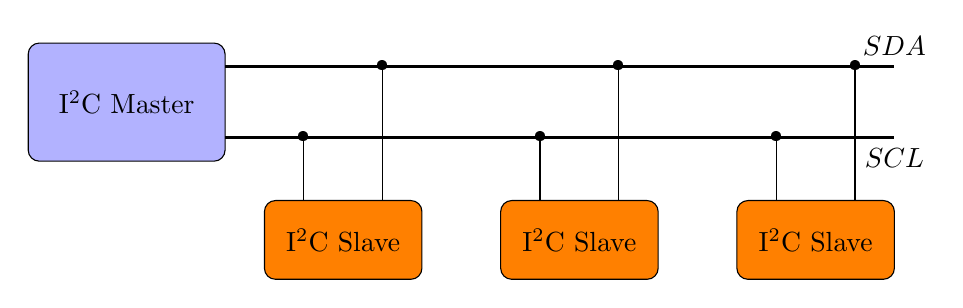
\begin{tikzpicture}
%    \draw[gray] (0,0) grid (11,3);
%    \foreach \x in {0,1,...,11}
%           \draw (\x cm,1pt) -- (\x cm,-1pt) node[anchor=north] {$\x$};
%    \foreach \y in {1,2,3}
%       \draw (1pt,\y cm) -- (-1pt,\y cm) node[anchor=east] {$\y$};

    %draw master and slave device
    \draw [rounded corners, fill=blue!30] (0, 1.5) rectangle (2.5,3) node[pos=.5] {I$^{2}$C Master};
    \foreach \x in {3,6,9}
    {
        \draw [rounded corners, fill=orange] (\x, 0) rectangle (\x+2,1) node[pos=.5] {I$^{2}$C Slave};
    }

    %draw circuit
    \draw[very thick] (2.5,1.8) -- (11,1.8) node[pos=1, below] {$SCL$};    %SCL
    \draw[very thick] (2.5,2.7) -- (11,2.7) node[pos=1, above] {$SDA$};    %SDA
    \foreach \x in {3.5, 6.5, 9.5}
    {
        \draw (\x, 1) -- (\x, 1.8);
        \node at (\x, 1.8) {\textbullet};
    }
    \foreach \x in {4.5, 7.5, 10.5}
    {
        \draw (\x, 1) -- (\x, 2.7);
        \node at (\x, 2.7) {\textbullet};
    }
\end{tikzpicture}

\end{document}
